\chapname = {MAAS in VENV - IV : Acquisition}

\chapter{\the\chapname}

After setting up the nodes and commissioning them, the next logical step is machine acquisition and deployment.

\section{User management}

One need to have a account to acuire a machine. An account can only be created by an admin. The account information can be managed in Users section in settings on the MAAS web interface(fig. 6.1).

\begin{figure}[!ht]
    \centering
    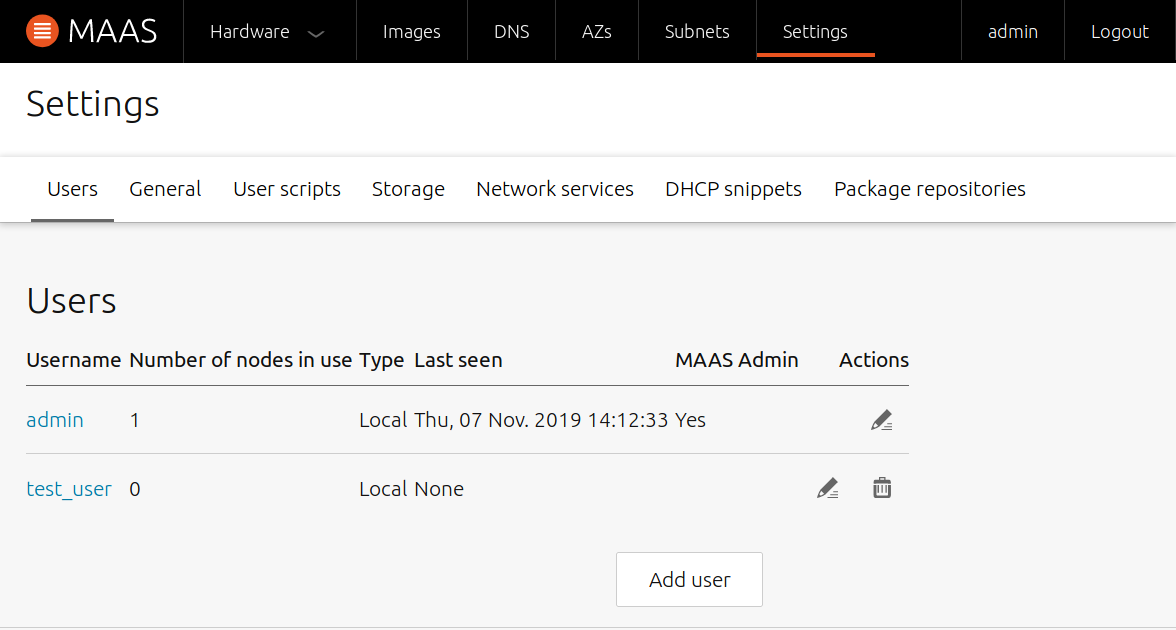
\includegraphics[width=0.7\textwidth]{images/6-1.png}
    \caption{User management}
\end{figure}

We will create a test user with no administrator privileges. 

\section{Acquiring machine}

Once a user login for the first time, they will be prompted to provide SSH keys (fig 6.2). Refer fig. 6.3 for generating a ssh key.

\begin{figure}[!ht]
    \centering
    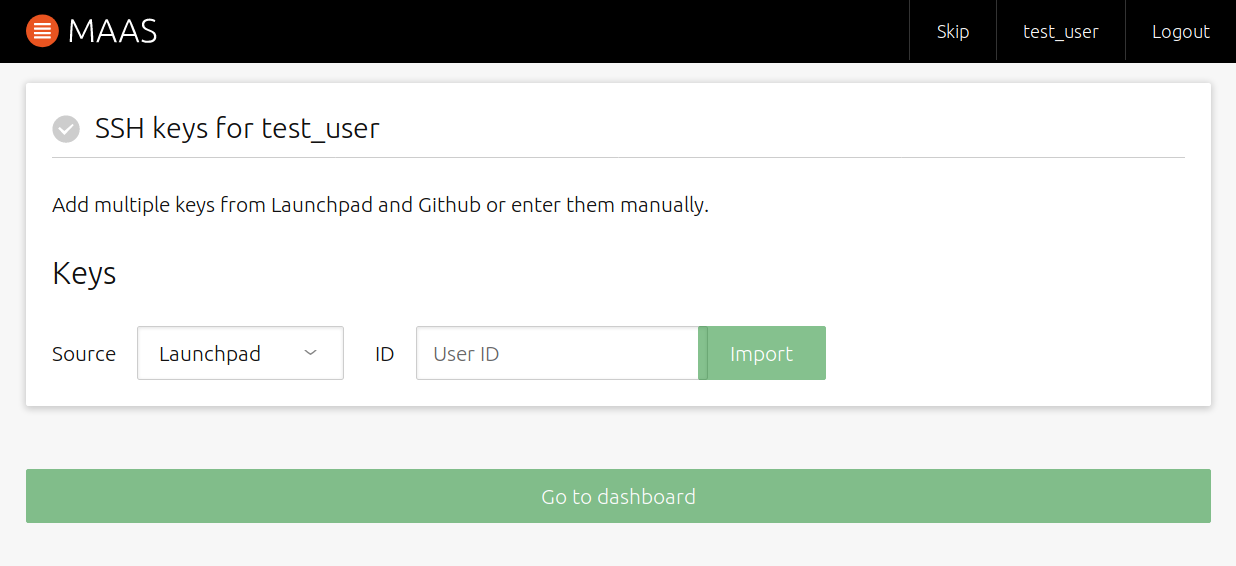
\includegraphics[width=0.7\textwidth]{images/6-2.png}
    \caption{Provide SSH keys}
\end{figure}


\begin{figure}[!ht]
    \centering
    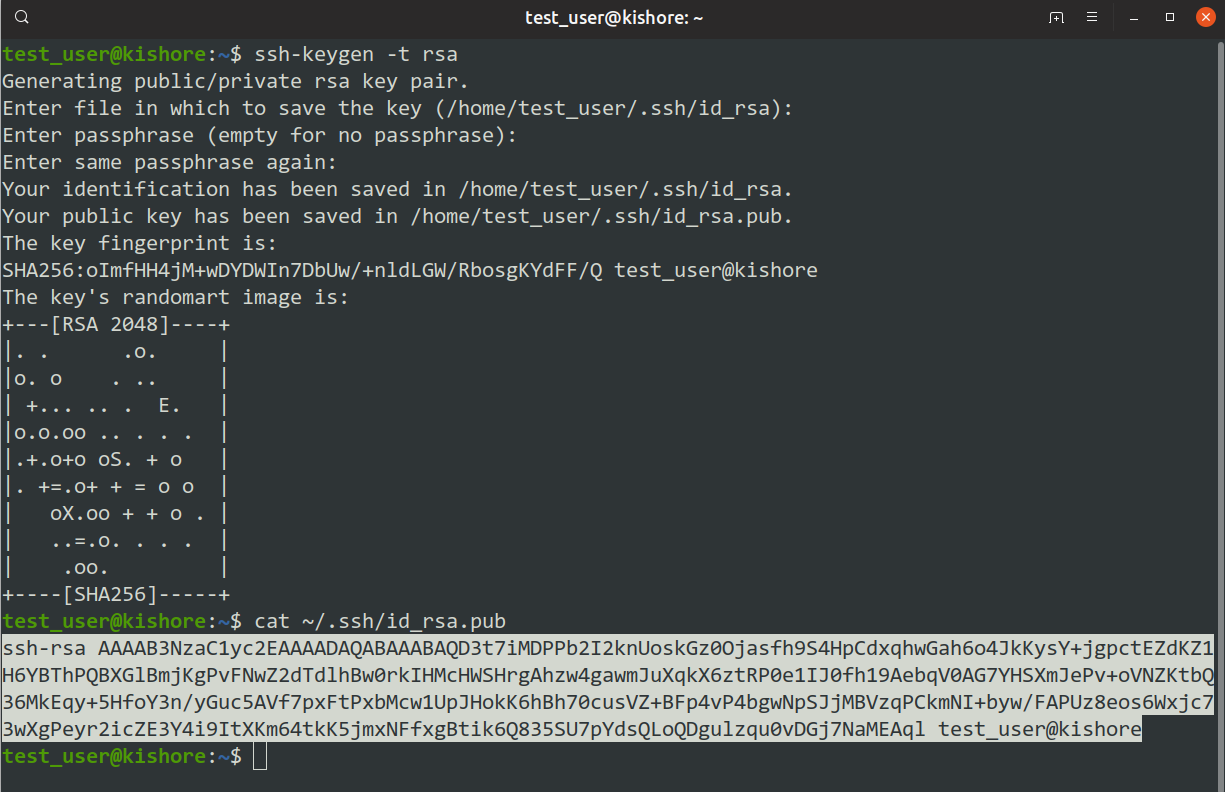
\includegraphics[width=0.7\textwidth]{images/6-3.png}
    \caption{Generating a ssh key}
\end{figure}

Copy the ssh key to the MAAS and proceed to the machines section where you will find the lists of the machines that is available for the user to manage. 

Important thing to note here is that the machines list may differ depending on whether the user has administrator privileges or not. The test\_user doesn't have administrator privileges and hence node0 is not visible to them as it is currently allocated to admin (fig. 6.4 \& 6.5).

\begin{figure}[!ht]
    \centering
    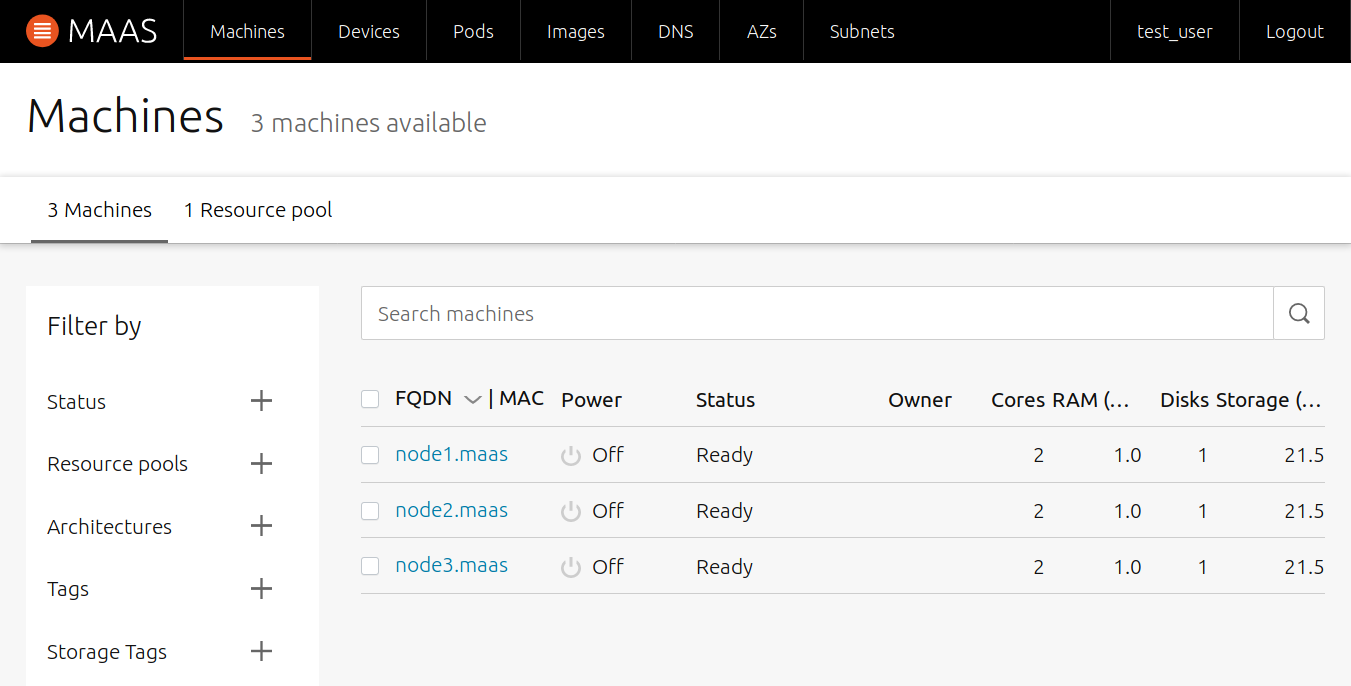
\includegraphics[width=0.7\textwidth]{images/6-4.png}
    \caption{Machine list seen by test\_user}
\end{figure}


\begin{figure}[!ht]
    \centering
    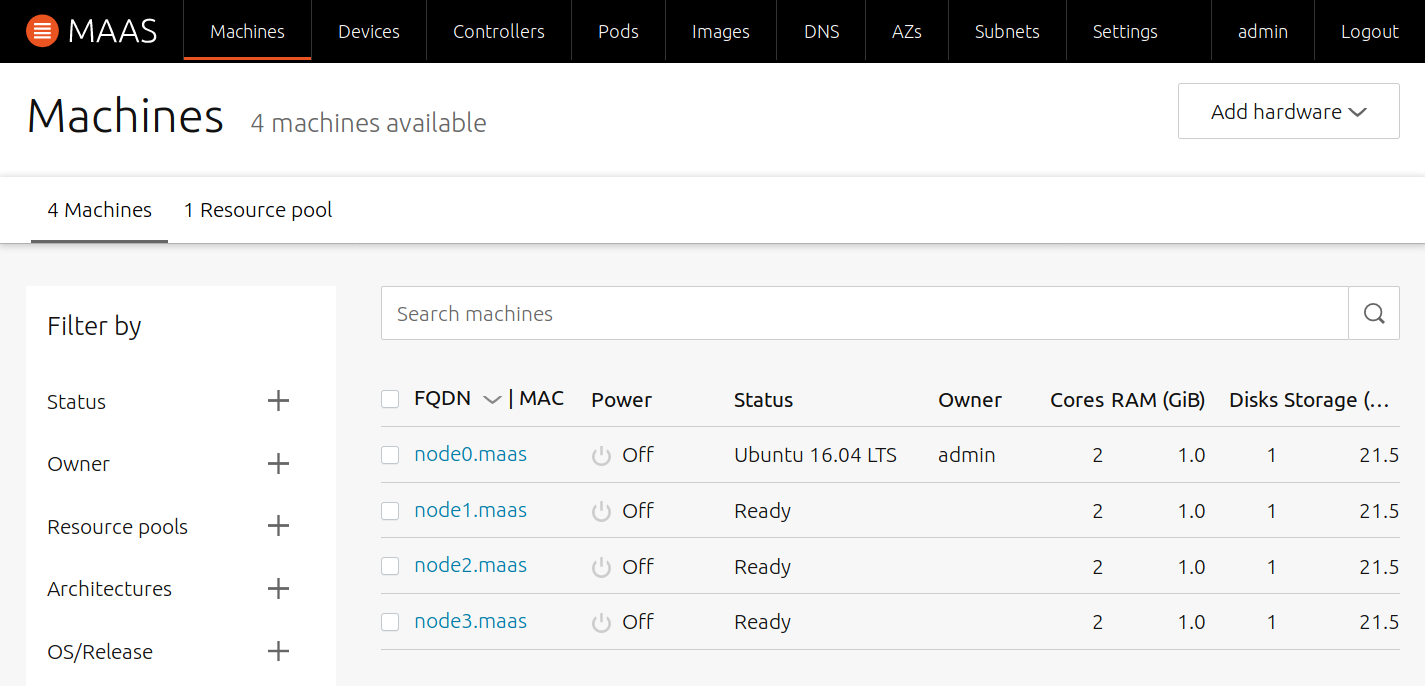
\includegraphics[width=0.7\textwidth]{images/6-5.png}
    \caption{Machine list seen by admin}
\end{figure}

Finally all the preparations are done and we are ready for machine acquisition and deployment. 

To acquire a machine just select a few machines from the list and choose acquire option from the take action menu(fig. 6.6).

\begin{figure}[!ht]
    \centering
    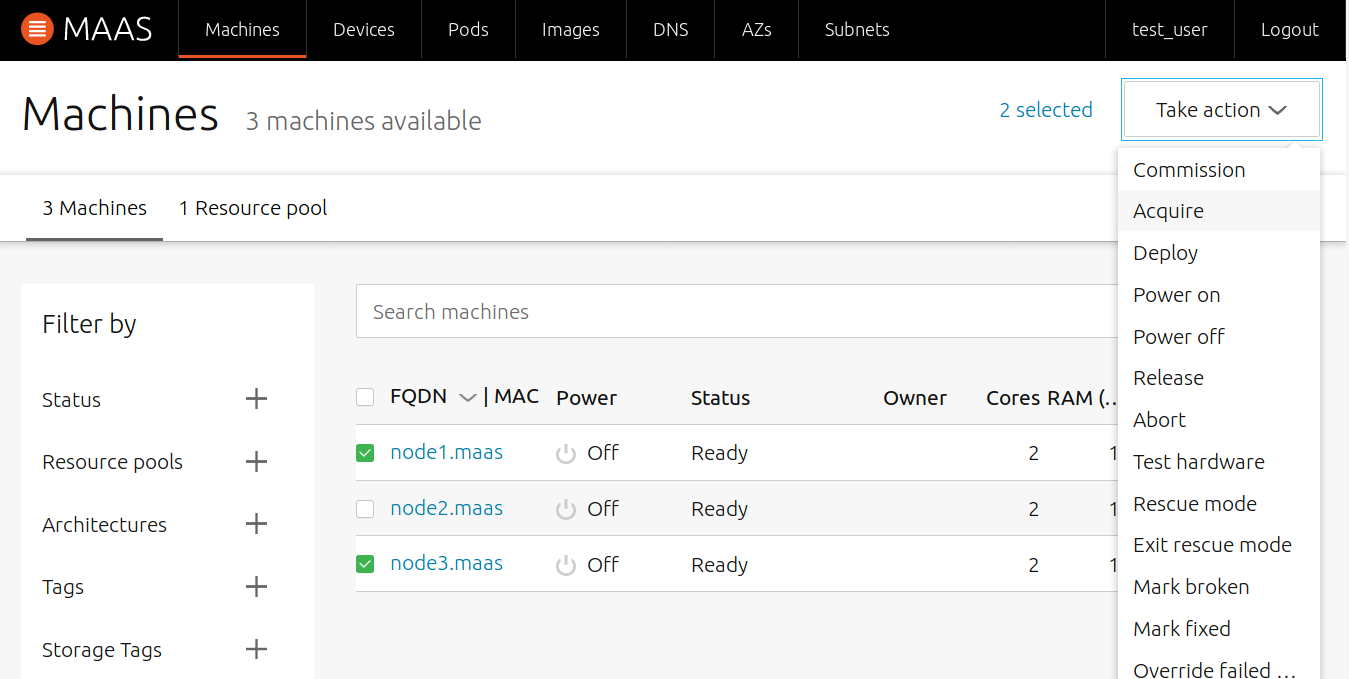
\includegraphics[width=0.7\textwidth]{images/6-6.png}
    \caption{test\_user acquiring node1 and node3}
\end{figure}

\begin{figure}[!ht]
    \centering
    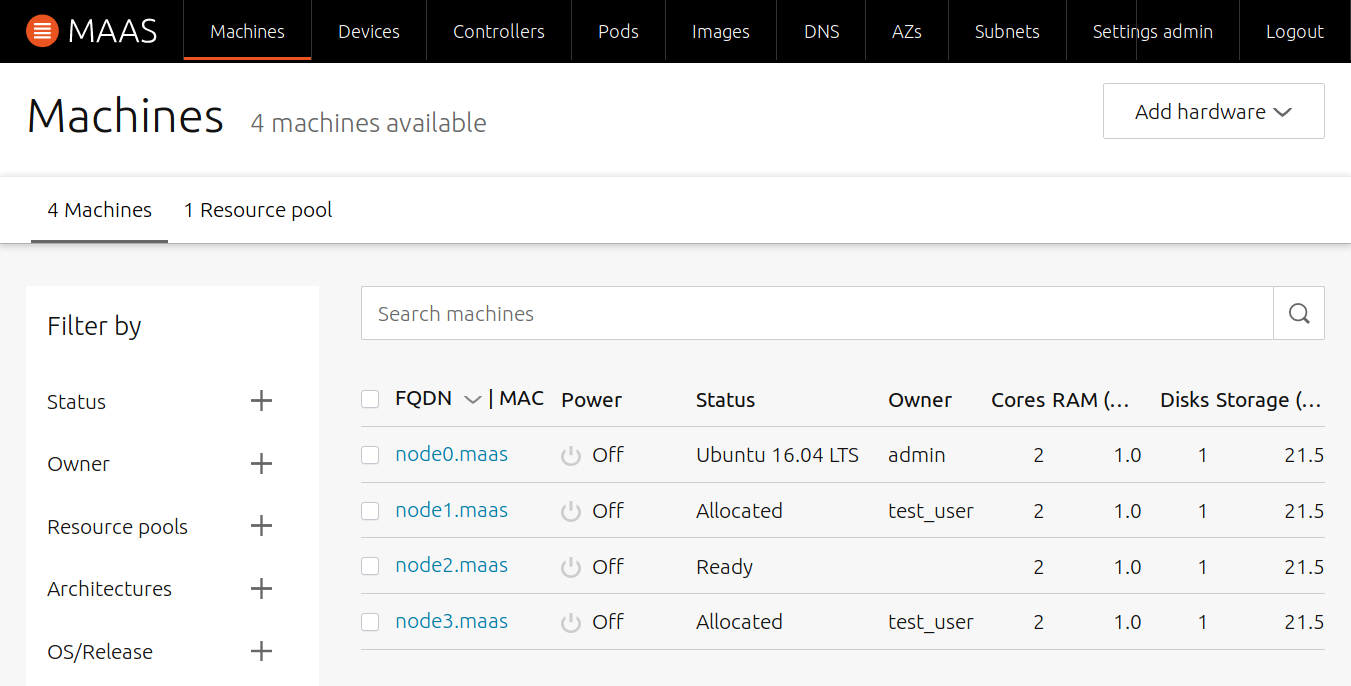
\includegraphics[width=0.7\textwidth]{images/6-7.png}
    \caption{admin can monitor status of nodes}
\end{figure}

\section{Deployment}

Once the node1 and node3 is acquired by test\_user, they can deploy an image to a machine. The deployment is straightforward just select the desired machine and under the take action menu select deploy option. They will be given a dropdown list of the images available for the deployment. Select an image and proceed. I am deploying one of the machines with ubuntu 14.04 image and other one with centos 6.


\begin{figure}[!ht]
    \centering
    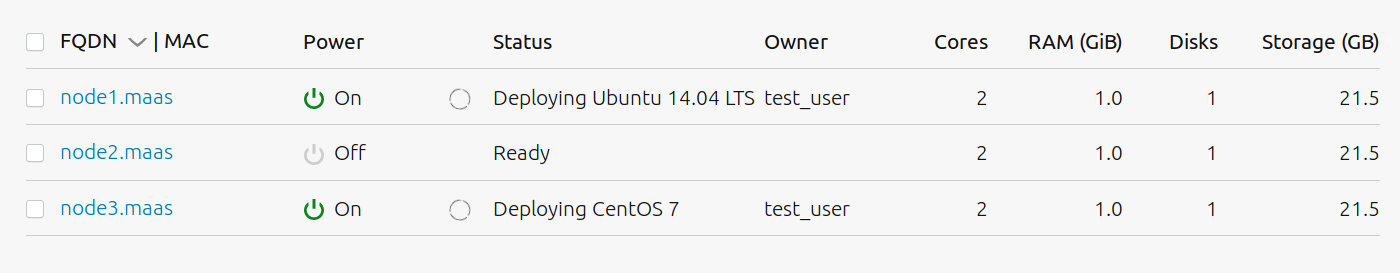
\includegraphics[width=0.8\textwidth]{images/6-8.png}
    \caption{Deployment}
\end{figure}

Once the deployment is finished the test\_user can ssh login to the machine. Given below are ssh commands for the ssh login to the machines:

(For ubuntu deployment) \$ ssh ubuntu@\textless IP\textgreater

(For centos deployment) \$ ssh centos@\textless IP\textgreater

IP address can be found from the interface menu for a node.

\begin{figure}[!ht]
    \centering
    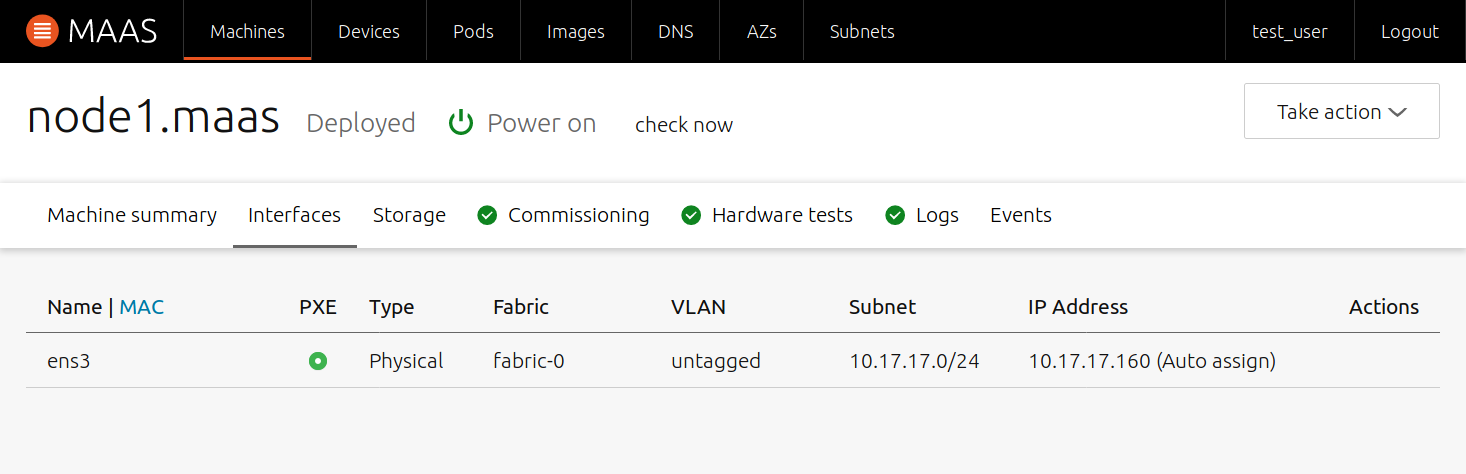
\includegraphics[width=0.8\textwidth]{images/6-9.png}
    \caption{Find IP address}
\end{figure}

Remember that the MAAS asked for the ssh key in the beginning and hence we won't be prompted any password(fig. 6.10).

\begin{figure}[!ht]
    \centering
    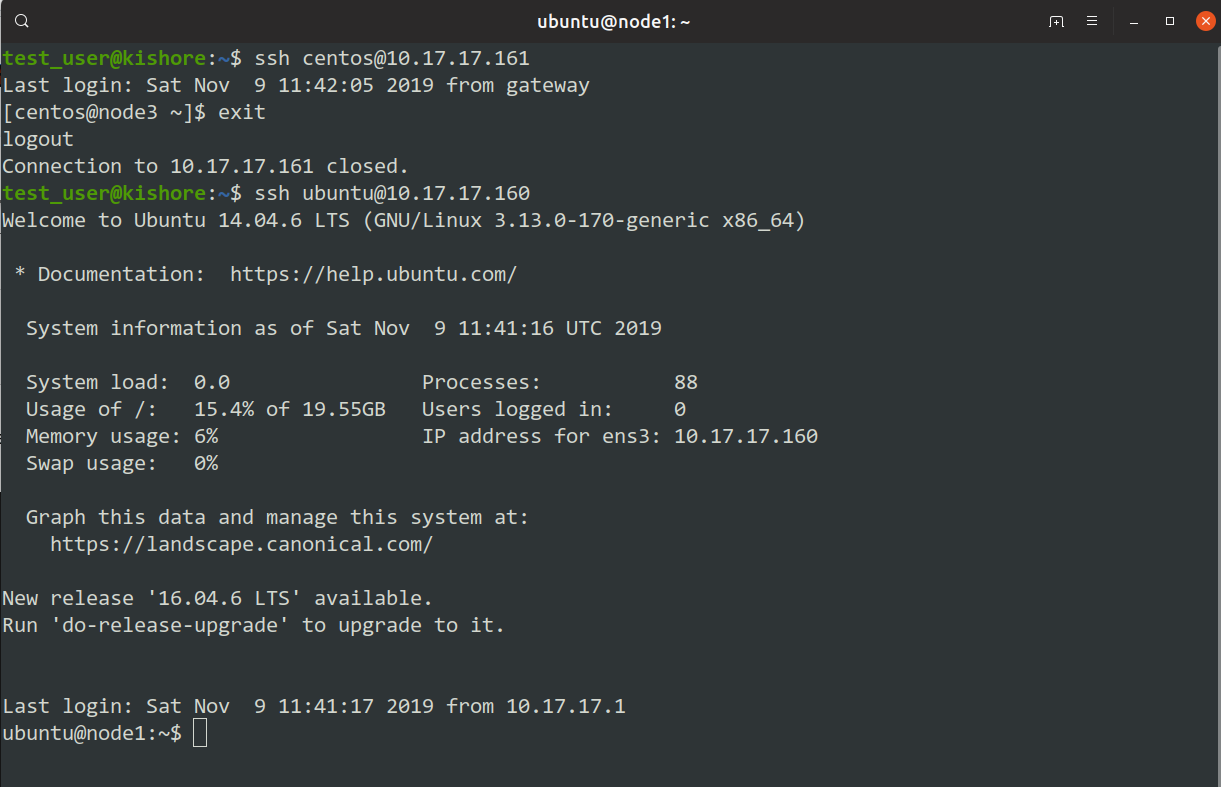
\includegraphics[width=0.7\textwidth]{images/6-10.png}
    \caption{Logging to the machines}
\end{figure}

\section{Conclusion}

This ends our journey with how to create a virtual MAAS based cloud environment. To summarise, we first created a virtual network and added a few virtual machines to it. Then we made one of the machines the controller which will act as the entry point for the users who want to interact with the cloud. Then we created a few virtual machines where the PXE boot is enabled. Then we commissioned them and performed basic hardware test. Finally we created a user to test the deployment.